\documentclass{article}
\usepackage{macro}
\usepackage{graphicx}
\graphicspath{ {./} }
\title{Policy Gradient Methods for Deep Reinforcement Learning}
\author{Hongshan Li}
\begin{document}
\maketitle

RL is big and rich, its history traces back to Pavlov's study on the 
psychology of animal learning (conditional response) back in 1902.
The expository article History of Reinforcement Learning (http://incompleteideas.net/book/first/ebook/node12.html) is a good resource to learn
how RL evolved in the last 100 years.

Policy Gradient Methods is a class of RL algorithms that directly 
learns a policy from interaction with the environment. In contrast,
to this, one can also learn a state value estimate of the current
state of the env and the candidate actions. This class of algorithms
is called Q-learning. 


\textbf{Review about setups in RL}
The objective of RL is to find a policy $\pi$ that gets the highest 
rewards from a \emph{Markov Decision Process}

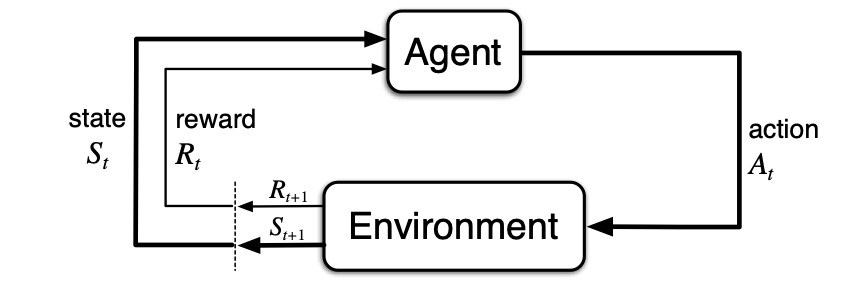
\includegraphics[width=8cm]{mdp}

At time step $t$, the env is at state $S_t$, the agent takes action 
$A_t$, the env transition into $S_{t+1}$ and the agent receives a 
reward of $R_{t+1}$. 

The critical assumption of MPD is
\begin{itemize}
    \item The transition probability $P(S_{t+1}, R_{t+1}|S_t, A_t)$ is
        independent from the history
    \item The agent's action does not alter the transition probability,
        i.e. $P(S_{t+1}, R_{t+1} | S_t, A_t)$ is the same whenver 
        the agent sees $S_t$ and takes action $A_t$
\end{itemize}

The transition probability $P(S_{t+1}, R_{t+1} | S_t, A_t)$ is call 
the \emph{model} of the env. The objective of RL is to find a
\emph{optimal policy}
(what action to take at $S_t$) that maximize the total reward

If $P(S_{t+1}, R_{t+1}|S_t, A_t) = 1$ for all $S$ and $A$, then we say
the env is deterministic, otherwise stochastic.

The total reward from time $t$ is 
\[
    G_t = R_{t+1} + R_{t+2} + \cdots + R_{T}
\]
The MDP terminates at $T$. 

To prioritize short term return over long term return, we use a 
discount factor $\gamma \in [0, 1]$ and define
\[
    G_t = R_{t+1} + \gamma R_{t+2} + \gamma^2 R_{t+3} + \cdots 
    + \gamma^k R_{t+k+1} + \cdots + \gamma^{T-t-1}R_{T}
\]

A few ways to think about the discount factor
\begin{itemize}
    \item prioritize short term reward
    \item A mathematical convenience for infinite episodic task; we 
        want $G_t$ to be a finite number even if the MDP never stops.
        \[
            \sum_{i=0}^{\infty} \gamma^i = \frac{1}{1-\gamma}
        \]
        so 
        \[
            G_t \le \frac{1}{1-\gamma} * R_{\max}
        \]
    \item a way to factor in the probability that agent dies. The agent 
        survives with prob $\gamma$ and die with prob $1 - \gamma$.
        i.e reward at time $t$ is 
        \[
            \gamma R_{t+1} + (1 - \gamma) * 0
        \]
\end{itemize}

Let $\mathscr{S}$ be the state space, and $\mathscr{A}$ the action space.
A \emph{deterministic policy} is a mapping 
\[
    \pi: \mathbb{S} \rightarrow \mathbb{A}
\]
and a \emph{stochastic} policy is a mapping
\[
    \pi: \mathbb{S} \rightarrow Dist( \mathbb{A} )
\]
where $Dist(\mathscr{ A })$ denote the space of probability distributions
over the action spaces.

Both deterministc env and determinsitc policy are special cases of their
stochastic counterparts.(all probability concentrate at 1 point). So 
we only address the stochastic cases in the rest of the note.

Suppose the agent's current policy is $\pi$, then at state $S_t$
$\pi$ yields a probability distribution over the action space
\[
    \pi(\cdot | S_t)
\]
from which the agent samples actions. 

So with the model of the env, we can write down the expected total 
reward if we follow the policy $\pi$. Assume the initial state is $s$
\[
    v_{\pi}(s) \definedas \E_{\pi}
\]


A fundamental difference supervised learning and RL is that data is 
completely determined before any training, whereas in RL data is
dynamically generated through interaction with the environment. 
This means the distribution of the data for SL is static and the 
distribution of data for RL changes as the agent learns. 

Talk about value iteration and policy iteration;
Talk about how tabular methods can be used to achieve
value/policy iteration;
Talk about why tabular method is not sufficient and function 
approximator;

then talk about parametrized policy and policy gradient theorem 



\textbf{REINFOCE}



% \biblio
History of Reinforcement Learning
http://incompleteideas.net/book/first/ebook/node12.html
\end{document}

